\documentclass{beamer}
\mode<presentation>{
  \usetheme{Boadilla}
  \usefonttheme[onlylarge]{structurebold}
  \usefonttheme[stillsansseriflarge]{serif}
  \setbeamerfont*{frametitle}{size=\normalsize,series=\bfseries}
  % \setbeamertemplate{navigation symbols}{}
  \setbeamercovered{transparent}
}
\usepackage[english]{babel}
\usepackage[latin1]{inputenc}
\usepackage{times}
\usepackage[T1]{fontenc}
\usepackage{amsmath}
\usepackage{amssymb}
\usepackage{esint}
\usepackage{hyperref}
\usepackage{tikz}
\usepackage{xkeyval}
\usepackage{xargs}
\usepackage{xcolor}
\usepackage{verbatim}
\usepackage{listings}
\usepackage{multimedia}
\usepackage{bm}
\usepackage{siunitx}
\usetikzlibrary{
  arrows,
  calc,
  decorations.pathmorphing,
  decorations.pathreplacing,
  decorations.markings,
  fadings,
  positioning,
  shapes,
  arrows.meta
}
\usepgfmodule{oo}

\pgfdeclareradialshading{glow2}{\pgfpoint{0cm}{0cm}}{
  color(0mm)=(white);
  color(2mm)=(white);
  color(8mm)=(black);
  color(10mm)=(black)
}
\pgfdeclareradialshading{glow}{\pgfpoint{0cm}{0cm}}{
  color(0mm)=(white);
  color(5mm)=(white);
  color(9mm)=(black);
  color(10mm)=(black)
}

\begin{tikzfadingfrompicture}[name=glow fading]
  \shade [shading=glow] (0,0) circle (1);
\end{tikzfadingfrompicture}

\begin{tikzfadingfrompicture}[name=glow2 fading]
  \shade [shading=glow2] (0,0) circle (1);
\end{tikzfadingfrompicture}

\mode<handout>{
  \usepackage{pgfpages}
  \pgfpagesuselayout{4 on 1}[a4paper,landscape,border shrink=5mm]
  \setbeamercolor{background canvas}{bg=black!10}
}

\newcommand\pgfmathsinandcos[3]{%
  \pgfmathsetmacro#1{sin(#3)}%
  \pgfmathsetmacro#2{cos(#3)}%
}
\newcommand\LongitudePlane[3][current plane]{%
  \pgfmathsinandcos\sinEl\cosEl{#2} % elevation
  \pgfmathsinandcos\sint\cost{#3} % azimuth
  \tikzset{#1/.estyle={cm={\cost,\sint*\sinEl,0,\cosEl,(0,0)}}}
}
\newcommand\LatitudePlane[3][current plane]{%
  \pgfmathsinandcos\sinEl\cosEl{#2} % elevation
  \pgfmathsinandcos\sint\cost{#3} % latitude
  \pgfmathsetmacro\yshift{\cosEl*\sint}
  \tikzset{#1/.estyle={cm={\cost,0,0,\cost*\sinEl,(0,\yshift)}}} %
}
\newcommand\DrawLongitudeCircle[2][1]{
  \LongitudePlane{\angEl}{#2}
  \tikzset{current plane/.prefix style={scale=#1}}
  % angle of "visibility"
  \pgfmathsetmacro\angVis{atan(sin(#2)*cos(\angEl)/sin(\angEl))} %
  \draw[current plane] (\angVis:1) arc (\angVis:\angVis+180:1);
  \draw[current plane,dashed] (\angVis-180:1) arc (\angVis-180:\angVis:1);
}
\newcommand\DrawLatitudeCircleArrow[2][1]{
  \LatitudePlane{\angEl}{#2}
  \tikzset{current plane/.prefix style={scale=#1}}
  \pgfmathsetmacro\sinVis{sin(#2)/cos(#2)*sin(\angEl)/cos(\angEl)}
  % angle of "visibility"
  \pgfmathsetmacro\angVis{asin(min(1,max(\sinVis,-1)))}
  \draw[current plane,decoration={markings, mark=at position 0.6 with {\arrow{<}}},postaction={decorate},line width=.6mm] (\angVis:1) arc (\angVis:-\angVis-180:1);
  \draw[current plane,dashed,line width=.6mm] (180-\angVis:1) arc (180-\angVis:\angVis:1);
}
\newcommand\DrawLatitudeCircle[2][1]{
  \LatitudePlane{\angEl}{#2}
  \tikzset{current plane/.prefix style={scale=#1}}
  \pgfmathsetmacro\sinVis{sin(#2)/cos(#2)*sin(\angEl)/cos(\angEl)}
  % angle of "visibility"
  \pgfmathsetmacro\angVis{asin(min(1,max(\sinVis,-1)))}
  \draw[current plane] (\angVis:1) arc (\angVis:-\angVis-180:1);
  \draw[current plane,dashed] (180-\angVis:1) arc (180-\angVis:\angVis:1);
}
\newcommand\coil[1]{
  {\rh * cos(\t * pi r)}, {\apart * (2 * #1 + \t) + \rv * sin(\t * pi r)}
}
\makeatletter
\define@key{DrawFromCenter}{style}[{->}]{
  \tikzset{DrawFromCenterPlane/.style={#1}}
}
\define@key{DrawFromCenter}{r}[1]{
  \def\@R{#1}
}
\define@key{DrawFromCenter}{center}[(0, 0)]{
  \def\@Center{#1}
}
\define@key{DrawFromCenter}{theta}[0]{
  \def\@Theta{#1}
}
\define@key{DrawFromCenter}{phi}[0]{
  \def\@Phi{#1}
}
\presetkeys{DrawFromCenter}{style, r, center, theta, phi}{}
\newcommand*\DrawFromCenter[1][]{
  \setkeys{DrawFromCenter}{#1}{
    \pgfmathsinandcos\sint\cost{\@Theta}
    \pgfmathsinandcos\sinp\cosp{\@Phi}
    \pgfmathsinandcos\sinA\cosA{\angEl}
    \pgfmathsetmacro\DX{\@R*\cost*\cosp}
    \pgfmathsetmacro\DY{\@R*(\cost*\sinp*\sinA+\sint*\cosA)}
    \draw[DrawFromCenterPlane] \@Center -- ++(\DX, \DY);
  }
}
\newcommand*\DrawFromCenterText[2][]{
  \setkeys{DrawFromCenter}{#1}{
    \pgfmathsinandcos\sint\cost{\@Theta}
    \pgfmathsinandcos\sinp\cosp{\@Phi}
    \pgfmathsinandcos\sinA\cosA{\angEl}
    \pgfmathsetmacro\DX{\@R*\cost*\cosp}
    \pgfmathsetmacro\DY{\@R*(\cost*\sinp*\sinA+\sint*\cosA)}
    \draw[DrawFromCenterPlane] \@Center -- ++(\DX, \DY) node {#2};
  }
}
\makeatother

% not mandatory, but I though it was better to set it blank
\setbeamertemplate{headline}{}
\def\beamer@entrycode{\vspace{-\headheight}}

\tikzstyle{snakearrow} = [decorate, decoration={pre length=0.2cm,
  post length=0.2cm, snake, amplitude=.4mm,
  segment length=2mm},thick, ->]

%% document-wide tikz options and styles

\tikzset{%
  % >=latex, % option for nice arrows
  inner sep=0pt,%
  outer sep=2pt,%
  mark coordinate/.style={inner sep=0pt,outer sep=0pt,minimum size=3pt,
    fill=black,circle}%
}
\tikzset{
  % Define standard arrow tip
  >=stealth',
  % Define style for boxes
  punkt/.style={
    rectangle,
    rounded corners,
    draw=black, very thick,
    text width=8em,
    minimum height=2.5em,
    text centered},
}

\tikzset{onslide/.code args={<#1>#2}{%
    \only<#1>{\pgfkeysalso{#2}}
    % \pgfkeysalso doesn't change the path
  }}
\tikzset{alt/.code args={<#1>#2#3}{%
    \alt<#1>{\pgfkeysalso{#2}}{\pgfkeysalso{#3}}
    % \pgfkeysalso doesn't change the path
  }}
\tikzset{temporal/.code args={<#1>#2#3#4}{%
    \temporal<#1>{\pgfkeysalso{#2}}{\pgfkeysalso{#3}}{\pgfkeysalso{#4}}
    % \pgfkeysalso doesn't change the path
  }}

\makeatletter
\newbox\@backgroundblock
\newenvironment{backgroundblock}[2]{%
  \global\setbox\@backgroundblock=\vbox\bgroup%
  \unvbox\@backgroundblock%
  \vbox to0pt\bgroup\vskip#2\hbox to0pt\bgroup\hskip#1\relax%
}{\egroup\egroup\egroup}
\addtobeamertemplate{background}{\box\@backgroundblock}{}
\makeatother

% \def\timeleft{15:00->14:55}

\title{Optics}
\date{Oct. 18, 2022}
\author{Yichao Yu}
\institute{Journal Club}

\ifpdf
  % Ensure reproducible output
  \pdfinfoomitdate=1
  \pdfsuppressptexinfo=-1
  \pdftrailerid{}
  \hypersetup{
    pdfcreator={},
    pdfproducer={}
  }
\fi

\begin{document}

{
  \begin{frame}{}
    \titlepage
  \end{frame}
}

\begin{frame}{Geometrical optics}
  \begin{center}
    \visible<1->{
      \textbf{Useful for $>90\%$ of calculation.}\\
    }
    \visible<2->{
      \begin{columns}
        \column{7cm}
        \begin{block}{Exceptions}
          \begin{itemize}
          \item Focus
          \item<3-> Long propagation
          \item<4-> Diffraction optical elements\\
            e.g. gratings.
          \end{itemize}
        \end{block}
      \end{columns}
    }
  \end{center}
\end{frame}

\begin{frame}{Ideal Lens}
  \begin{center}
    \begin{tikzpicture}
      \visible<-7>{
        \draw[red, line width=1.5] (-2.25, 0.8) -- (4.5, -1.6);
        \draw[red, line width=1.5] (-2.25, 0.8) -- (0, -1.6) -- (4.5, -1.6);
        \draw[red, line width=1.5] (-2.25, 0.8) -- (0, 0.8) -- (4.5, -1.6);

        \draw[dashed, line width=2] (-5, 0) -- (5, 0);
        \draw[<->,>=stealth, line width=1.5] (0, 2) -- (0, -2);
        \fill (-1.5, 0) circle (0.1) node[below=0.16] {F};
        \fill (1.5, 0) circle (0.1) node[below=0.16] {F};
        \draw[->, line width=1] (-2.25, 0) -- (-2.25, 0.8);
        \draw[->, line width=2] (4.5, 0) -- (4.5, -1.6);

        \node[below=0.05] at (-0.6, 0) {$f$};
        \node[below=0.02] at (0.8, 0) {$f$};
      }
      \visible<8->{
        \draw[red, line width=1.5] (-3.05, 0.8) -- (-0.8, 0);
        \draw[red, line width=1.5] (0.2, 0) -- (4.7, -1.6);
        \draw[red, line width=1.5] (-3.05, 0.8) -- (-0.8, -1.6);
        \draw[red, line width=1.5] (0.2, -1.6) -- (4.7, -1.6);
        \draw[red, line width=1.5] (-3.05, 0.8) -- (-0.8, 0.8);
        \draw[red, line width=1.5] (0.2, 0.8) -- (4.7, -1.6);

        \draw[dashed, line width=2] (-5, 0) -- (5, 0);
        \draw[dashed, line width=1.5] (-0.8, -2) -- (-0.8, 2) node[above] {$H_1$};
        \draw[dashed, line width=1.5] (0.2, -2) -- (0.2, 2) node[above] {$H_2$};
        \fill (-2.3, 0) circle (0.1) node[below=0.16] {F};
        \fill (1.7, 0) circle (0.1) node[below=0.16] {F};
        \draw[->, line width=1] (-3.05, 0) -- (-3.05, 0.8);
        \draw[->, line width=2] (4.7, 0) -- (4.7, -1.6);

        \node[below=0.05] at (-1.4, 0) {$f$};
        \node[below=0.02] at (1.0, 0) {$f$};
      }

      \visible<2-3>{
        \draw[green!70!black,decoration={brace,amplitude=10pt},decorate,line width=1]
        (-2.2, 0.9) -- node[above=0.32] {$u$} (-0.05, 0.9);
        \draw[green!70!black,decoration={brace,amplitude=10pt},decorate,line width=1]
        (0.05, 0.9) -- node[above=0.32] {$v$} (4.45, 0.9);
        \draw[dashed, line width=1.5, opacity=0.3] (4.5, 0.8) -- (4.5, 0);
      }

      \visible<4-5>{
        \draw[blue!70!black,decoration={brace,mirror,amplitude=5pt},
        decorate,line width=1]
        (-2.25, -0.6) -- node[below=0.2] {$x_1$} (-1.5, -0.6);
        \draw[blue!70!black,decoration={brace,amplitude=10pt},
        decorate,line width=1]
        (1.5, 0.2) -- node[above=0.32] {$x_2$} (4.5, 0.2);
      }
      \visible<2-3>{
        \node[green!70!black] at (0, -2.7) {$\dfrac{1}{u}+\dfrac{1}{v}=\dfrac{1}{f}$};
        \visible<3>{
          \node[green!70!black] at (0, -3.7) {$M=\dfrac{v}{u}$};
        }
      }
      \visible<4-5>{
        \node[blue!70!black] at (0, -2.7) {$x_1x_2=f^2$};
        \visible<5>{
          \node[blue!70!black] at (0, -3.7) {$M=\dfrac{f}{x_1}=\dfrac{x_2}{f}=\sqrt{\dfrac{x_2}{x_1}}$};
        }
      }
      \visible<6-7>{
        \node[below,align=center,text width=6cm] at (0, -2.3) {
          \begin{tabular}{rl}
            Conjugate plane:\!\!&\!\!Perfect image under ray optics\\
            \visible<7->{Principal planes:}\!\!&\!\!\visible<7->{Conjugate plane where $M=1$}
          \end{tabular}
        };
      }
    \end{tikzpicture}
  \end{center}
\end{frame}

\begin{frame}{Spherical lens}
  \begin{center}
    \begin{tikzpicture}
      \draw[dashed, line width=2] (-5, 0) -- (5, 0);
      \visible<-3>{
        \draw[line width=0.8,fill=cyan!60!blue,fill opacity=0.3]
        (0, -2) arc (-11.536959032815489:11.536959032815489:10)
        arc ({180-23.578178478201835}:{180+23.578178478201835}:5);
      }
      \visible<4>{
        \draw[line width=0.8,fill=cyan!60!blue,fill opacity=0.3]
        (0, -2) -- (0, 2)
        arc ({180-23.578178478201835}:{180+23.578178478201835}:5);
      }

      \visible<1>{
        \draw[line width=0.8,dashed]
        (0, 2) arc (11.536959032815489:18:10);
        \path[line width=0.8,dashed]
        (0, 2) arc (11.536959032815489:16:10) coordinate (R1);
        \draw[<-,>=stealth,line width=1.2] (R1) -- node[sloped, above] {$R_1$} ++(18:-1);

        \draw[line width=0.8,dashed]
        (0, 2) arc (180-23.578178478201835:180-30.5:10);
        \path[line width=0.8,dashed]
        (0, 2) arc (180-23.578178478201835:180-28:10) coordinate (R2);
        \draw[<-,>=stealth,line width=1.2] (R2) -- node[sloped, above] {$R_2$} ++(-28:1);
      }

      \visible<2-4>{
        \draw[red, line width=1.5] (-5, 0.3) -- (0, 0.3) -- (5, -0.2);
        \draw[red, line width=1.5] (-5, -0.3) -- (0, -0.3) -- (5, 0.2);
      }
      \visible<3>{
        \draw[red!20!orange, line width=1] (-5, 0.6) -- (0, 0.6) -- (2.7, 0) -- (4.5, -0.4);
        \draw[red!20!orange, line width=1] (-5, -0.6) -- (0, -0.6) -- (2.7, 0) -- (4.5, 0.4);

        \draw[red!20!orange, line width=1] (-5, 0.9) -- (0, 0.9) -- (2.4, 0) -- (4.0, -0.6);
        \draw[red!20!orange, line width=1] (-5, -0.9) -- (0, -0.9) -- (2.4, 0) -- (4.0, 0.6);

        \draw[red!20!orange, line width=1] (-5, 1.2) -- (0, 1.2) -- (2.1, 0) -- (3.5, -0.8);
        \draw[red!20!orange, line width=1] (-5, -1.2) -- (0, -1.2) -- (2.1, 0) -- (3.5, 0.8);
      }
      \visible<2-4>{
        \fill (3, 0) circle (0.08) node[below=0.16] {F};
      }
    \end{tikzpicture}
  \end{center}
\end{frame}

\begin{frame}{Aspherical lens}
  \begin{center}
    \begin{columns}
      \column{3cm}
      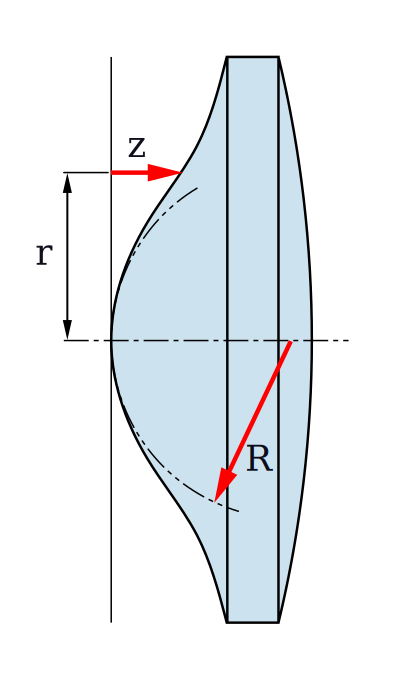
\includegraphics[width=2.5cm]{imgs/Asphere.pdf}
      \column{6cm}
      \visible<2->{
        \begin{block}{Use cases}
          \begin{itemize}
          \item Collimation
          \item Fiber coupling
          \end{itemize}
        \end{block}
      }
    \end{columns}
  \end{center}
\end{frame}

\begin{frame}{Other lens types}
  \begin{center}
    \begin{columns}
      \column{5.2cm}
      \visible<1->{
        \begin{block}{Reflective}
          \begin{itemize}
          \item No chromatic shift
          \item Can be aspherical
          \item More difficult beam path layout
          \end{itemize}
        \end{block}
      }
      \column{5.2cm}
      \visible<2->{
        \begin{block}{Lens set}
          \begin{itemize}
          \item Could fix chromatic shift
          \item Could fix monochromatic aberration
          \item Better surface quality
          \item May not be UV compatible
          \end{itemize}
        \end{block}
      }
    \end{columns}
  \end{center}
\end{frame}

\end{document}
